%
% -- Manlio Modugno

\documentclass{beamer} 
\usepackage{eulervm}
%\usepackage{booktabs}
\usepackage{listings}
\usepackage{bold-extra}
\usepackage{cancel}
\usepackage{fancybox}
\usepackage{soul}
\usepackage[english]{babel}
\usepackage[utf8]{inputenc}
\usepackage{hyperref}
\usepackage{amsmath}
%\hypersetup{colorlinks=true,urlcolor=blue}

\newcommand{\codefont}{\fontsize{6}{8}\selectfont}
\lstset{language=[Sharp]C, 
captionpos=b, 
frame=lines,
lineskip= 1pt, %space between lines
basicstyle=\codefont, 
keywordstyle=\color{blue}, 
commentstyle=\color{green}, 
stringstyle=\color{red}, 
numbers=left, 
numberstyle=\tiny, 
stepnumber=2,
numbersep=5pt,
breaklines=true, 
breakatwhitespace=false,
showstringspaces=false,
frame=single,
tabsize=2,
emph={double,bool,int,unsigned,char,true,false,void},
emphstyle=\color{blue},
emph={Assert,Test},
emphstyle=\color{red},
emph={[2]\using,\#define,\#ifdef,\#endif},
emphstyle={[2]\color{blue}}
}


\mode<presentation>
\definecolor{title_color}{RGB}{2,128,181} 
\usetheme{Ilmenau}
\usecolortheme[named=title_color]{structure}
\setbeamercolor{palette quaternary}{use=structure,fg=black,bg=white} %header footer color
\useoutertheme[subsection=false]{smoothbars}
\setbeamercovered{transparent}
\setbeamertemplate{navigation symbols}{}
\setbeamerfont{subsection in toc}{size=\scriptsize}

\title{The Single Responsibility Principle}
\author{Manlio Modugno}
\institute[GMTechnologies] 

\date[]{The Single Responsibility Principle}

\subject{}

\graphicspath{{img/}}
\pgfdeclareimage[height=0.6cm]{mfg-logo}{img/mfgLogo}
\logo{\pgfuseimage{mfg-logo}}

%
% Content start
%
\begin{document}
\begin{frame}
  \titlepage
\end{frame}

\begin{frame}
  \frametitle{Argomenti Trattati}
  \tableofcontents
\end{frame}


\section{Intro}
\subsection{Intro}
\begin{frame}
  \frametitle{Intro}
  \begin{itemize}
	\item<+-> \textbf{Cohesion}: is strictly correlated to SRP...
	\item<+-> a first definition is ``functional relatedness of the elements of a module''
	\item<+-> ..here the principle is seen as ``the forces that cause a module, or a class, to change ''
   \end{itemize}
\end{frame}

\begin{frame}
  \frametitle{Definition}
  \begin{itemize}
	\item<+-> def: \textbf{A Class Should Have Only One Reason To Change (!)}
   \end{itemize}
\end{frame}

\subsection{Motivation}
\begin{frame}
  \frametitle{Motivation: more responsibilities $ \rightarrow $ more reasons to change}
  \begin{itemize}
	\item<+-> Why it's so important to separate different responsibilities in different classes..?
	\item<+-> ..because every responsibility it's an axis of change.. 
	\item<+-> ..When  the  requirements  change,  that change will be manifest through a change in responsibility amongst the classes..
	\item<+-> ..when a class has more responsibilities, it has more than one reason to change
	\item<+-> If a class has more than one responsibility, then the responsibilities become coupled
	\item<+-> ..a change to a responsibility can break another one (in the same class).. 
	\item<+-> Redeployments.. but real lost time is in design phase / implementation
   \end{itemize}
\end{frame}

\begin{frame}
  \frametitle{Motivation: example}
    \textit{Rectangle} has more than one responsibility: \textit{draw()} and \textit{area()} \\
    \bigbreak
	\fbox{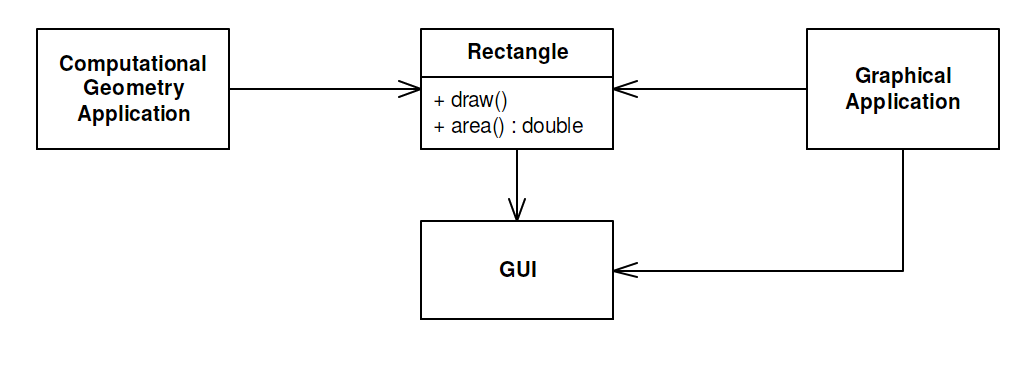
\includegraphics[scale=0.3]{badResp}}
\end{frame}

\begin{frame}
  \frametitle{Motivation: example}
  \begin{itemize}
	\item<+-> Two different applications use \textit{Rectangle}..
	\item<+-> ..one does computational and uses \textit{Rectangle} to do some math. 
	\item<+-> ..the other is merely graphic in nature..
	\item<+-> \textit{Rectangle} class has two responsibilities so it violates SRP
	\item<+-> If a class has more than one responsibility, then the responsibilities become coupled
	\item<+-> ..a change to a responsibility can break another one (in the same class).. 
   \end{itemize}
\end{frame}

\subsection{What is a Responsibility?}
\begin{frame}
  \frametitle{What is a Responsibility?}
  \begin{itemize}
	\item<+-> def: \textbf{A reason for change}
	\item<+-> ..if more than one motive exists for a class for change.. 
	\item<+-> ..that class has more than one responsibility
   \end{itemize}
\end{frame}

\begin{frame}[containsverbatim]
	\frametitle{What is a Responsibility?}
	To spot more than one responsibility can be hard.. we tend to group ``similar things'' \\
	\begin{lstlisting}
	public interface Modem{
		void Dial(string pno);
		void Hangup();
		void Send(char c);
		char Recv();
	}
	\end{lstlisting}
	Here, for example, there are two responsibilities.. \textit{Connection Management} and \textit{Data Communication}
\end{frame}

\subsection{How to identify responsibilities?}
\begin{frame}
  \frametitle{How to identify responsibilities?}
  \begin{itemize}
	\item<+-> How to proceed?... Should these responsibilities be separated?
	\item<+-> It' a trade off between \textbf{Rigidity} and \textbf{Needless Complexity}..
	\item<+-> Keep in mind that ``An axis of change is only an axis of change if the changes
actually occurr.. \textbf{It is not wise to apply the SRP, or any other principle, if there is no symptom}''
	\item<+-> (To feel that symptom it's not so simple sometime)
   \end{itemize}
\end{frame}

\begin{frame}
  \frametitle{Audience}
  \begin{itemize}
	\item<+-> A way to identify clearly a responsibility is to analyze the audience of the class / module..
	\item<+-> Audience can be defined as the actors belonging to a particular roles.. 
	\item<+-> Actors are sources of change for a responsibility (i.e. a family of functions), they manifest their needs during time...
	\item<+-> More actors $ \rightarrow $ probably more responsibilities... 
   \end{itemize}
\end{frame}

\subsection{Conclusion}
\begin{frame}
  \frametitle{Conclusion}
  \begin{itemize}
	\item<+-> SRP is one of the simplest of the principles, and one of the hardest to get right (i.e. achieving simplicity can be very tricky)
	\item<+-> Conjoining responsibilities is something that we do naturally..
	\item<+-> Finding and separating those responsibilities from one another is much of what software design is really about
   \end{itemize}
\end{frame}
\end{document}
